\chapter{\textit{Combined Process for Continuous Experimentation}}
\label{apdx:processo-erthal}

Este apêndice apresenta o processo combinado de experimentação proposto por \citeonline{erthal_characterization_2023}, ilustrado nas Figuras \ref{fig:erthal-process-a}, \ref{fig:erthal-process-b} e \ref{fig:erthal-process-c}. O diagrama foi segmentado em três partes para garantir a legibilidade de todas as fases, artefatos e atividades. As setas que conectam as figuras foram identificadas por letras em ordem alfabética, facilitando a compreensão do modelo como um todo.

\clearpage
\begin{landscape}
    \begin{figure}[p]
        \centering
        \caption{\textit{A Combined Process for Continuous Experimentation (Parte 1 de 3)}}
        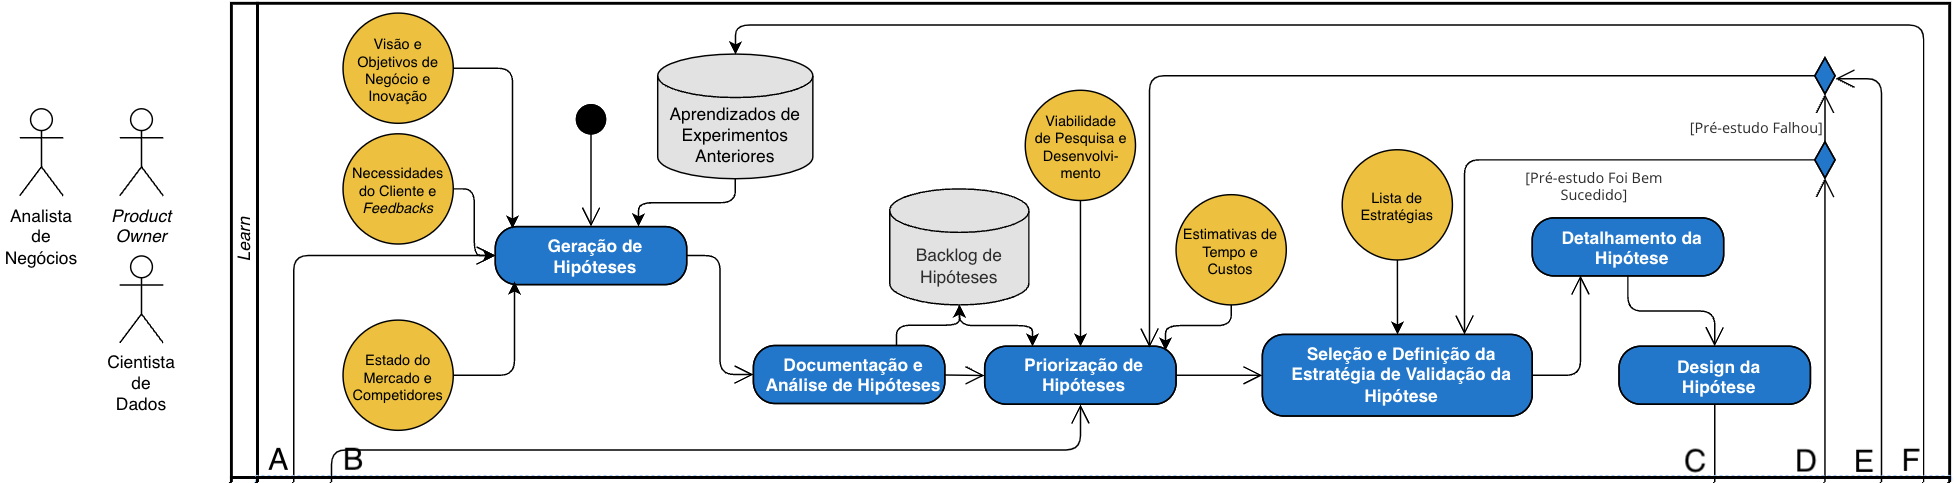
\includegraphics[width=1\linewidth]{figuras/processo_erthal_a.png}
        \text{Fonte: Adaptado de \citeonline{erthal_characterization_2023}}
        \label{fig:erthal-process-a}
    \end{figure}
\end{landscape}


\clearpage
\begin{landscape}
    \begin{figure}[p]
        \centering
        \caption{\textit{A Combined Process for Continuous Experimentation (Parte 2 de 3)}}
        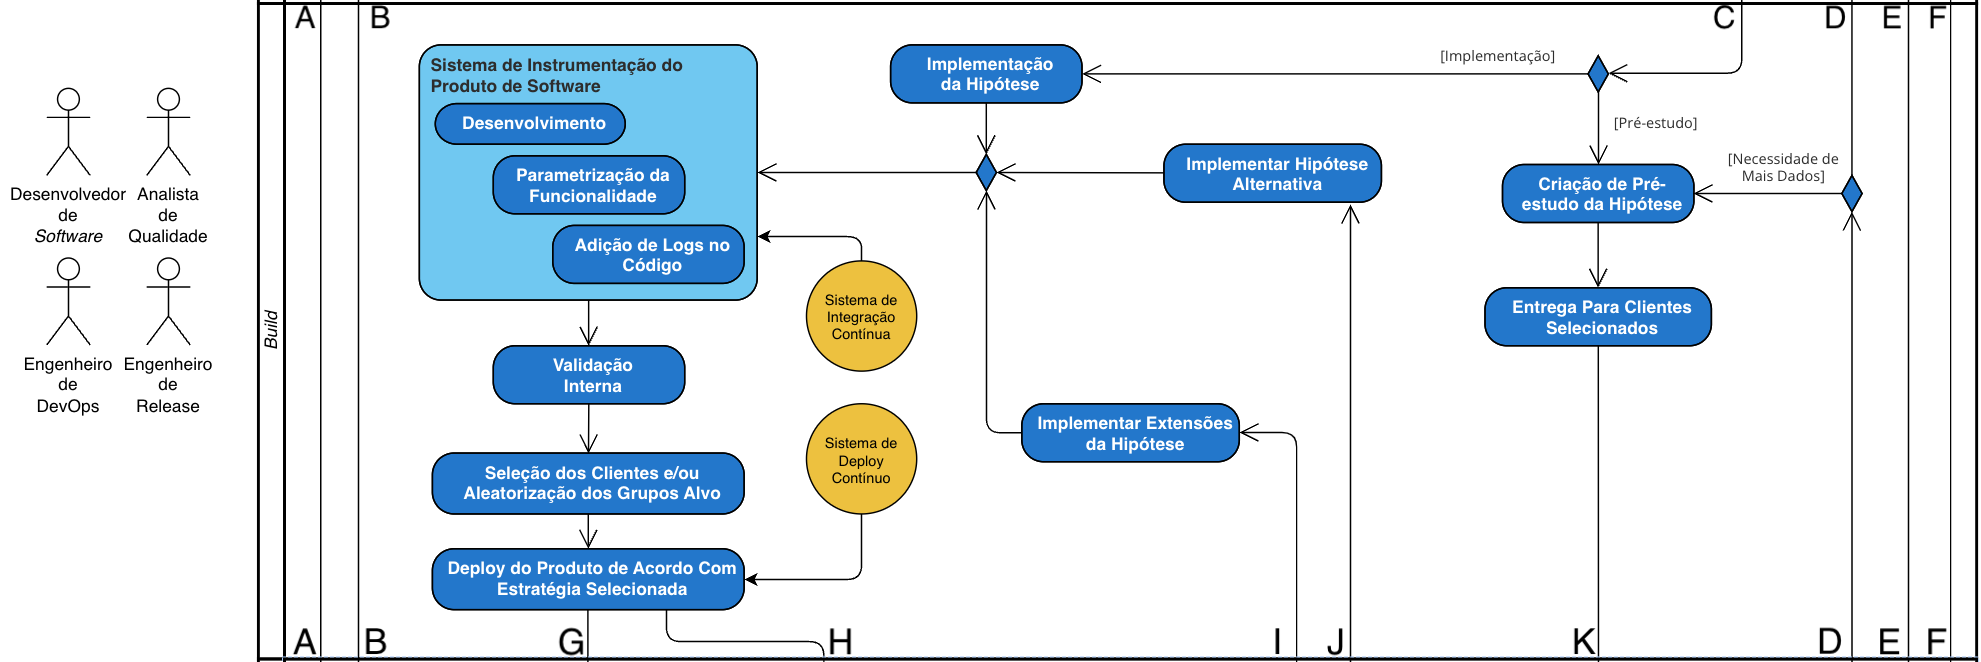
\includegraphics[width=1\linewidth]{figuras/processo_erthal_b.png}
        \text{Fonte: Adaptado de \citeonline{erthal_characterization_2023}}
        \label{fig:erthal-process-b}
    \end{figure}
\end{landscape}


\clearpage
\begin{landscape}
    \begin{figure}[p]
        \centering
        \caption{\textit{A Combined Process for Continuous Experimentation (Parte 3 de 3)}}
        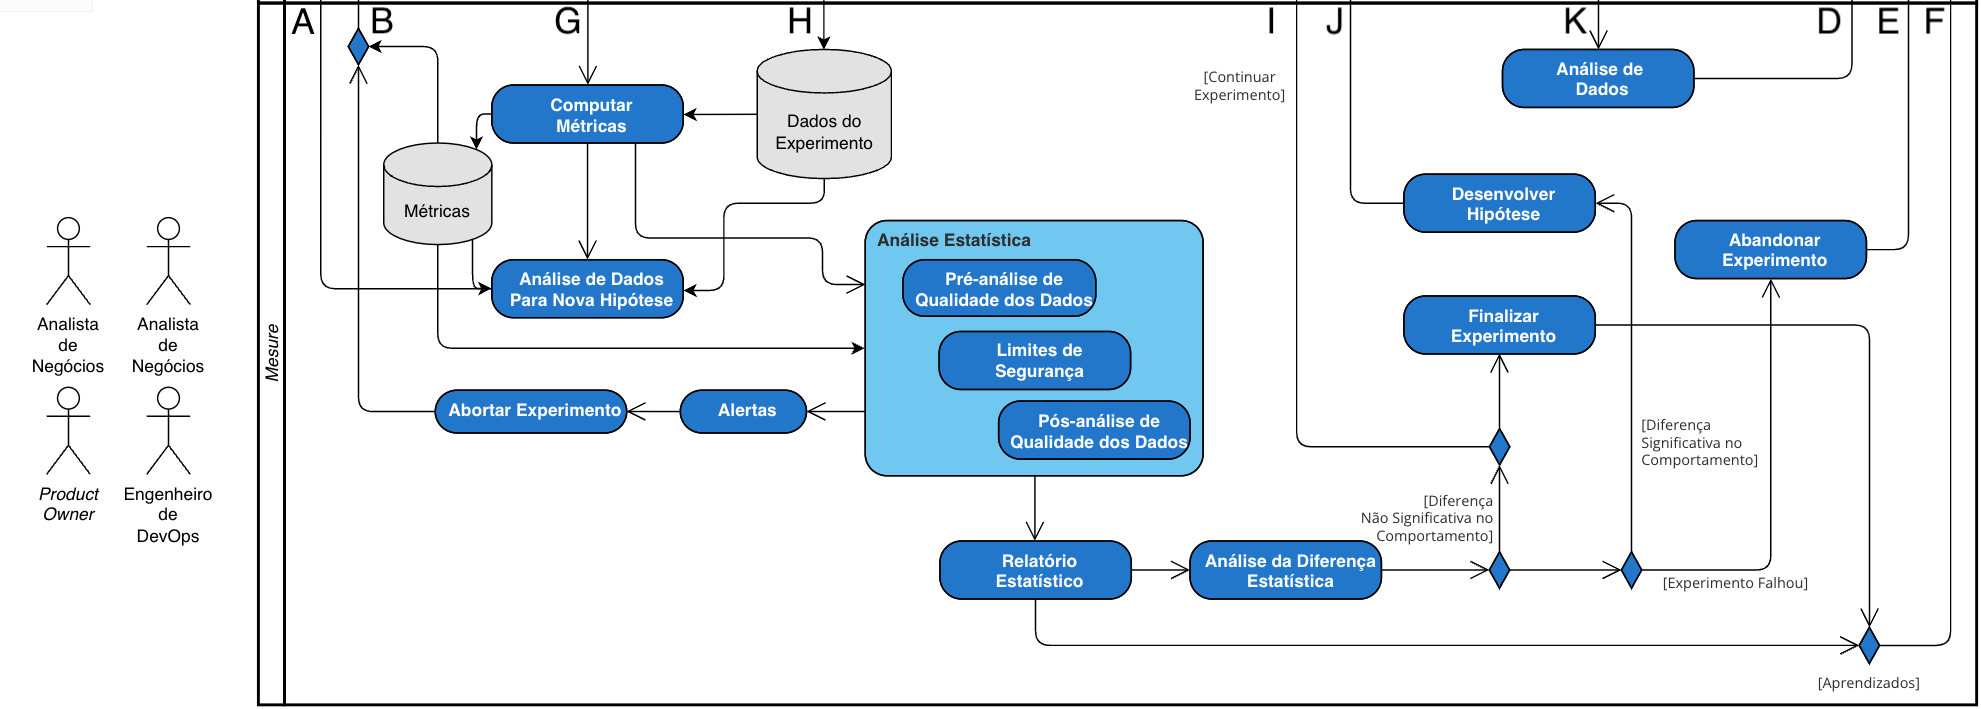
\includegraphics[width=1\linewidth]{figuras/processo_erthal_c.png}
        \text{Fonte: Adaptado de \citeonline{erthal_characterization_2023}}
        \label{fig:erthal-process-c}
    \end{figure}
\end{landscape}
